\documentclass{article}
\input{curvenote.def}

% colors for hyperlinks
\hypersetup{colorlinks=true, allcolors=blue}

[# if options.curvenote_logo_with_link #]
% We've included a Curvenote logo linking back to your online article based on the options you selected
\newcommand{\logo}{
  \href{[-doc.oxalink-]}{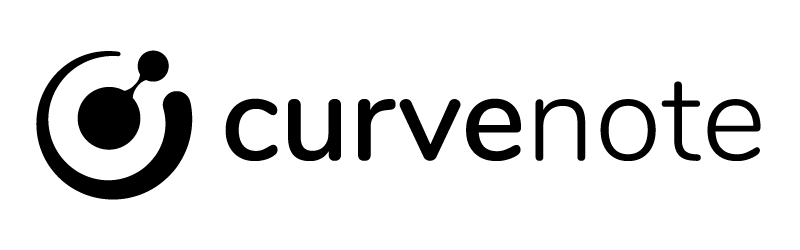
\includegraphics[width=2cm]{curvenote.png}}
}
[# endif #]

\title{[-doc.title-]}

\author{[-doc.authors|map(attribute="name")|join(" \\and ")-]}

\newdate{articleDate}{[-doc.date.day-]}{[-doc.date.month-]}{[-doc.date.year-]}
\date{\displaydate{articleDate}}

\begin{document}
\maketitle
[# if tagged.abstract #]\begin{abstract}[-tagged.abstract-]\end{abstract}[# endif #]
[# if options.curvenote_logo_with_link #]
\begin{center}\logo\end{center}
[# endif #]

[# if options.footnote_link #]
% Optional footnote with a link back to the online version of your article
\newcommand{\documentnote}[1]{{%
  \let\thempfn\relax% Remove footnote number printing mechanism
  \footnotetext[0]{\emph{#1}}% Print footnote text
}}
\documentnote{Available online at:\\ \href{[-doc.oxalink-]}{[-doc.oxalink-]}}
[# endif #]

[-CONTENT-]
\bibliography{main}
\end{document}
